%! TEX root = ../main.tex
\documentclass[main]{subfiles}

\begin{document}



\section{Teamenverの検証}
% textlint-disable
\begin{enumerate}
    \item 検証方法と結果\\
        アプリケーション開発の自主演習を用いた対照実験を行い,Teamenverを使用することでどのような効果があるのかを検証した.
        Teamenverを使用するチームと使用しないチームに分け,それぞれで同じアプリケーションを開発する.
        その後,アンケートをとり,次の項目について評価した: 
        (項目1)ライブラリの選択肢の多さ・初心者にとっての選択難易度,信頼や互換性のあるバージョンのライブラリの選定に関して
        (項目2)複数人開発でのライブラリ選定の意図の共有とメンバーの納得度に関して
        (項目3)知識の共有と保存に関して
        (項目4)チームとして開発環境構築することの難しさに関して
        特にチーム間で差が顕著であった項目1,3の結果は図\ref{fig:result}の通りである.
        
        \begin{figure}[h]
            \centering
            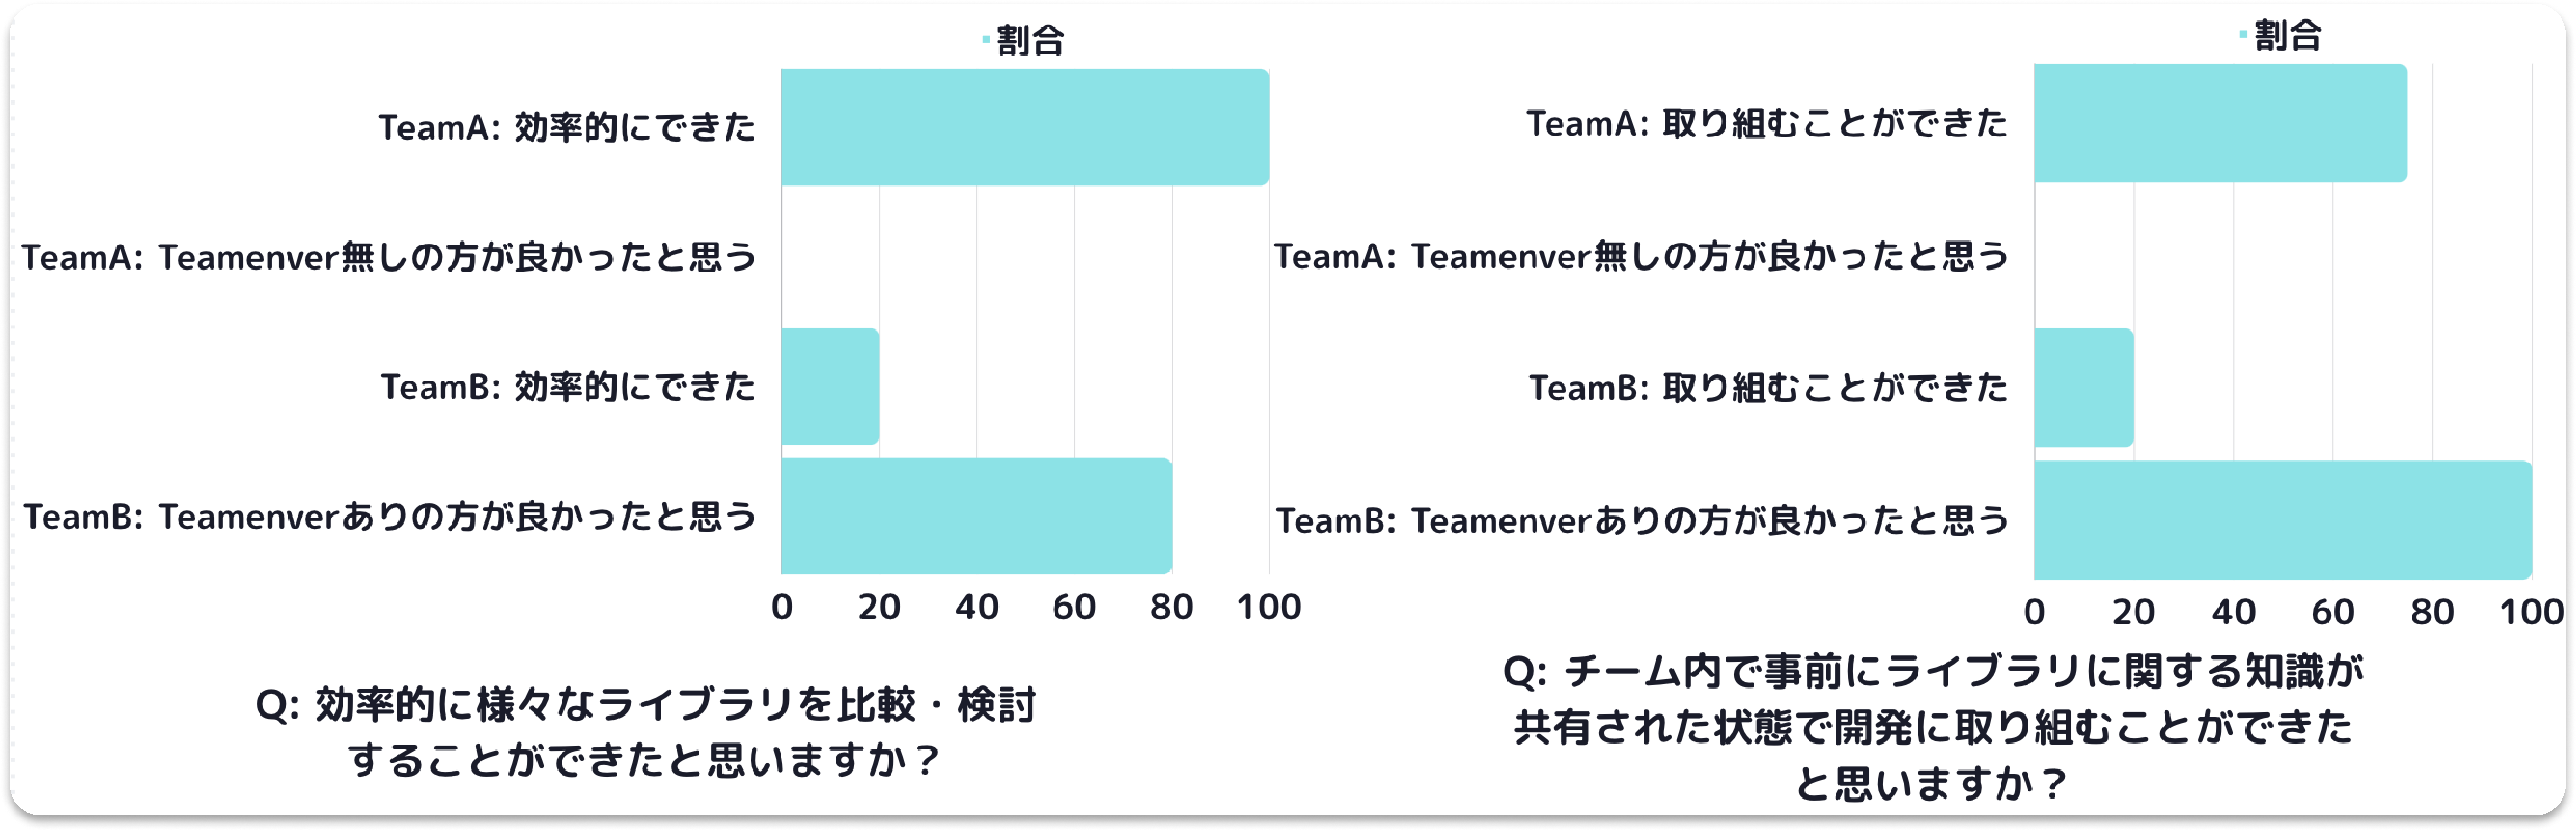
\includegraphics[keepaspectratio,width=1.1\linewidth]{../figures/result.pdf}
            \caption{項目1,3に関する質問の回答結果}
            \label{fig:result}
        \end{figure}
        
    \item 考察\\
            特に,ライブラリ選定の効率化と知識の共有に関しては,Teamenver未使用チームとの比較においてその効果が顕著であり,
        Teamenverの使用により,参加者が適切なライブラリを選択しやすくなり,
        チーム内での意見の一致や納得感を高めることができたと示されている.
\end{enumerate}
% textlint-enable

\end{document}

